\documentclass[10pt]{ctexart}
\usepackage{morelull}
\usepackage{enumerate}
\usepackage{bm}
\usepackage{makecell}
\usepackage{xcolor}
\usepackage{graphicx}
\usepackage{subfigure}
\usepackage{framed}%包中有添加文字背景色命令shaded
\colorlet{shadecolor}{MaterialBlue50}
\usepackage{tabularx}
\usepackage{multicol}  
\usepackage{multirow}
\usepackage{indentfirst}
\usepackage{amsmath,amssymb,amsthm,bm,bbding,pifont,dsfont}
\usepackage{mathtools}
\newcommand{\abs}[1]{\left| #1 \right|}
\usepackage{caption}
\captionsetup[figure]{labelfont={bf},labelformat={default},labelsep=period,name={图}}
%定义选择题选项
\newcommand{\onech}[4]{
\renewcommand\arraystretch{1.4}
\begin{tabularx}{\linewidth}{XXXX}
\setlength\tabcolsep{0pt}
(A) #1 & (B) #2 & (C) #3 & (D) #4 \\
\end{tabularx}
\unskip \unskip}
\newcommand{\twoch}[4]{
\renewcommand\arraystretch{1.4}
\begin{tabularx}{\linewidth}{XX}
\setlength\tabcolsep{0pt}
(A) #1 & (B) #2 \\
(C) #3 & (D) #4
\end{tabularx}
\unskip \unskip}

\title{模型研究系列 \quad 手拉手全等模型}
\author{一粒沙\\安徽省霍邱县龙潭中心校}
\date{\today}



\begin{document}
\maketitle
\tableofcontents


\section{什么是手拉手模型?}
所谓手拉手模型是指顶角相等,且有公共顶点的两个等腰三角形组成的图形,从中可以得到一个经典的全等模型:因为顶点相连的四条边,形象地可以看作两双手,所以通常称为“手拉手模型”。常见的有等边三角形共顶点,等腰直角三角形共顶点,正方形共顶点等几种,如下图所示。

\section{手拉手模型的类型}
\subsection{一般等腰三角形手拉手}
\begin{minipage}{0.4\textwidth}
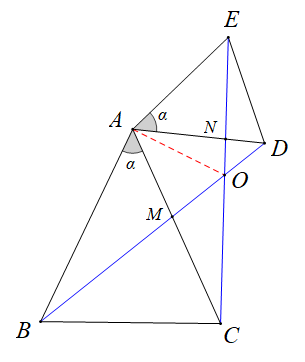
\includegraphics[scale=0.6]{figure/shoulashou01}
\end{minipage}
\begin{minipage}{0.6\textwidth}
  结论\ding{192}:\textcolor{red}{$\triangle ABD\cong \triangle ACE$};\\
  结论\ding{193}:\textcolor{red}{$BD=CE$};\\
  结论\ding{194}:\textcolor{red}{$\angle BOC=\angle BAC=\alpha$};\\
  结论\ding{195}:\textcolor{red}{$OA$平分$\angle BOE$};\\
  结论\ding{196}:\textcolor{red}{$\triangle ABM\sim \triangle OCM,\triangle AEM\sim \triangle ODN$};\\
   结论\ding{197}:\textcolor{red}{点$A,B,C,O$四点共圆,点$A,E,D,O$四点共圆}.
\end{minipage}
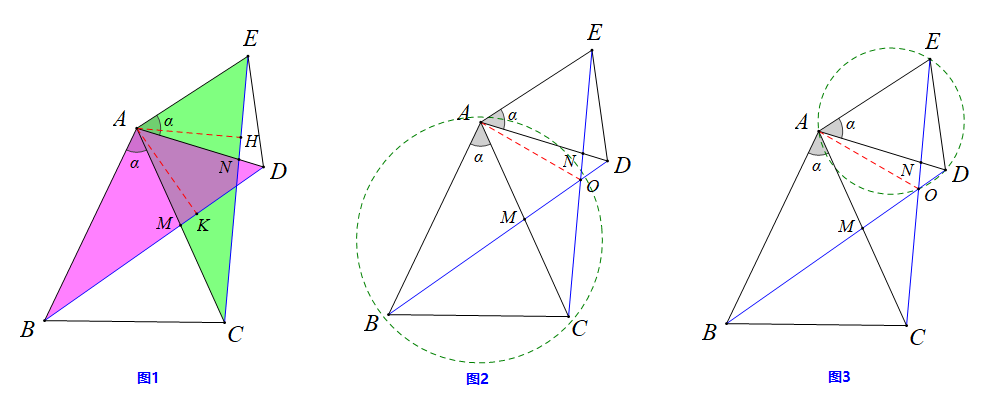
\includegraphics[scale=0.6]{figure/shoulashou02}
\subsection{等边三角形手拉手}
如图,直线$AB$的同侧作$\triangle ABD$和$\triangle BCE$都为等边三角形,连接$AE,CD$,二者交点为$H$,则有以下结论成立:

\begin{minipage}{0.4\textwidth}
	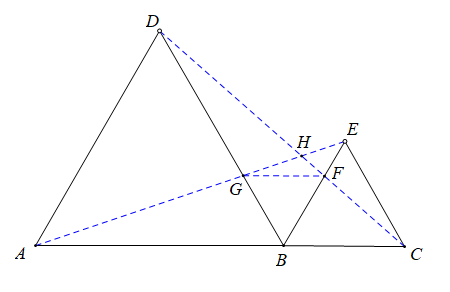
\includegraphics[scale=0.6]{figure/shoulashou03}
\end{minipage}
\begin{minipage}{0.6\textwidth}
 结论\ding{192}:\textcolor{red}{$\triangle ABE\cong \triangle DBC$};\\
结论\ding{193}:\textcolor{red}{$AE=DC$};\\
结论\ding{194}:\textcolor{red}{$\angle DHA=60^\circ$};\\
结论\ding{195}:\textcolor{red}{$\triangle AGB\cong \triangle DFB;\triangle EGB\cong \triangle CFB$};\\
结论\ding{196}:\textcolor{red}{连接$GF,\triangle BGF$是等边三角形};\\
结论\ding{197}:\textcolor{red}{$GF//AC$};\\
结论\ding{198}:\textcolor{red}{连接$HB$,$HB$平分$\angle AHC$};\\
结论\ding{199}:\textcolor{red}{$HC=HB+HE;HA=HC+HD$};\\
结论\ding{200}:\textcolor{red}{$\triangle DHG\sim \triangle ABG;\triangle EHF\sim \triangle CBF$};\\
结论\ding{201}:\textcolor{red}{点$A,B,H,D$四点共圆,点$C,B,H,E$四点共圆}.
\end{minipage}
\subsection{正方形手拉手}
\begin{minipage}{0.6\textwidth}
如图,四边形$ABCD$和四边形$CEFG$均为正方形,连接$BE,DG$,则有以下结论:

结论\ding{192}:\textcolor{red}{$\triangle BCE\cong \triangle DCG$};\\
结论\ding{193}:\textcolor{red}{$BE=DG,BE\perp DG$}.
\end{minipage}
\begin{minipage}{0.4\textwidth}
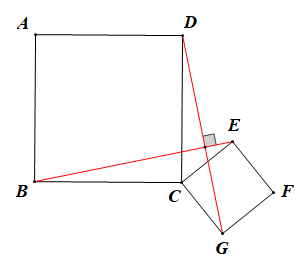
\includegraphics[scale=0.7]{figure/shoulashou04}
\end{minipage}

\section{习题演练}


\end{document}